\chapter{Tinker软件及算法介绍}
\label{cha:chapter03}

Tinker作为一台服务型机器人,一切设计都是为实现功能服务的。而编写软件
则是实现功能的直接手段。近几十年,一代代程序员和学者们为程序的开发
的管理提出了一个又一个理论,各式各样的开发方式和管理范式层出不穷,但真正
面对实际项目时,人员的分配,时间的管理,甚至硬件的掣肘无处不在。这些制约
笔者作为机器人队的主力程序员深有体会。本文作为Tinker机器人设计的客观描述
论文无意对项目管理这种不太容易客观表述的内容进行长篇的论述,但是笔者
深深的希望本文的读者能够在阅读本章关于软件设计及算法选型的内容中意识
到:程序的编写从来不以单一性能的最优为目的,而是在平衡整体功能的完成和系统
稳定性过程中的产物。代码的美丽与优雅固然可贵,但是无法实现需求的程序就是
一摊牛屎。

\section{软件设计概览}

本节主要大致讲述Tinker需要实现的基本功能以及将基本功能串联的控制逻辑的
实现。并且大致介绍一下Tinker搭载的各种主要传感器及它们的主要性能参数。
具体的方案及方案演进将在下一节进行详尽的展开。

\subsection{基本功能概览}

基础功能是支撑机器人完成复杂任务的基石,按照机器人领域的研究方向和习惯约定,
可以将机器人的功能大致的划分为4个主要方面。

\begin{itemize}
  \item 导航:建图、定位、路径规划与避障
  \item 抓取:机械臂运动规划与避障
  \item 感知:主要为基于视觉及RBGD的人脸检测、物体识别、及人类与物品的追踪
  \item 语音交互:主要为语音识别以及语音生成,以及简单的自然语言处理
\end{itemize}

这几大方向在学术界都有自己完善发展,社区中也各自有相当可用的几种开源方案。
但是将这些基本功能妥善的实现并且开放相应的功能接口供主控逻辑调用以完成
复杂的功能仍非易事。Tinker的开发过程中,每一种基本功能都经过了至少2版
的迭代,方案也几经更替,除了算法表现和稳定性的考量外,cpu和显卡占用,代码
开放性,社区成熟度等等因素都有着巨大的影响。

\subsection{控制逻辑的演进}
\label{sec:logic}

RoboCup@Home赛场上完成的任务本质上就是机器人通过调用几大基础功能实现
状态的转移,其间发生的结果处理以及异常管理功能其实都可以通过一个类似状态
机的机制来处理。基于这一思想,新版Tinker早期使用了ROS社区一个比较出名
的状态机控制包smach进行功能调用,完成主控逻辑的编写。

smach是一个较成熟的使用python编写的状态机控制仓库。它不但提供了完善的
状态命名、转移、分层分块机制,还显式的提供了良好的异常处理机制(如图\ref{fig:smach}
所示)。早期的
Tinker控制逻辑几乎完全依赖于smach实现,甚至整机的软件上电控制都由
smach编写。但是在经过反复的测试后smach的缺陷很快暴露出来,首先,Tinker
使用的很多基础功能是由c++编写的,在smach中想要直接调用他们不太现实,
需要额外开发python的wrapper或者使用ros的消息通信机制来调用他们,这
在客观上大大的增加了编码的工作量,且引入了非常多的bug,降低了系统的
稳定性。其次,使用python编码变成了一个门槛,将很多同学拦在开发之外,python
近几年是软件界的新宠,受到广大程序员及学者的追捧,但是不得不承认我校非
计算机专业的很多院系对同学们提供的编程教育是滞后的。相当多非计算机专业
且无计算机竞赛背景的同学刚加入机器人队时几乎完全不会写python,学习成本
也不太低。综合上述两个原因,除已经经过反复测试异常稳定的部分外,目前Tinker
大部分新编写的逻辑都是由c++编写的,只在开发简单的辅助工具或者脚本时才
使用python或者shell语言编写。

\begin{figure}[h] % use float package if you want it here
  \centering
  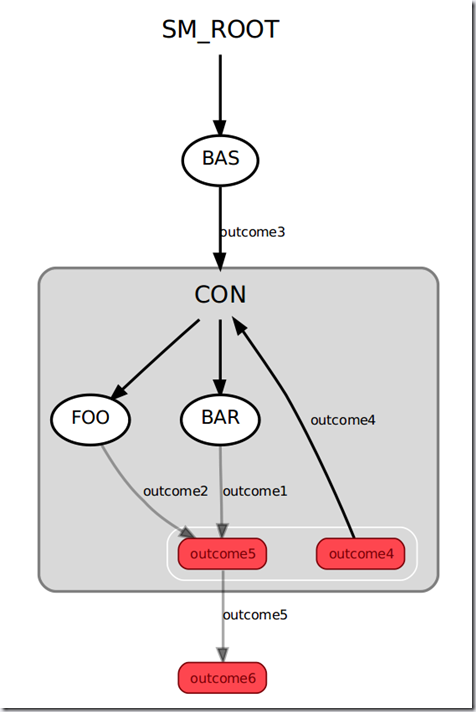
\includegraphics[width=.4\linewidth]{smach.png}
  \caption{smach的典型状态图}
  \label{fig:smach}
\end{figure}

当然c++编写会引入新的问题,比如c++可使用的功能性的包较少,包管理也几乎没有,
进行异常处理时非常麻烦等等。但是同完成功能协调队员合作比起来,这些问题
机器人团队也只能暂时忍耐,并不断寻求新的解决方案了。

\subsection{编码规范与版本控制}

在\ref{sec:logic}节中本文曾简短的探讨过开发语言的问题,以及python在
机器人开发过程中的劣势。事实上除了上述所说的困难外,使用python编写软件
还存在一个比较致命的缺陷,那就是python缺乏严格的类型检查机制。和c及c++
不同,python这种脚本语言缺乏“编译器”这个重要角色。这就导致在开发过程
中少了一个重要的约束,当项目合作的人员增多,代码开始膨胀的时候,相当多
的函数参数开始返回约定的规范之外的数据(这是程序员的惰性决定的),机器人
队没有条件像现代软件企业那样为研发的同学提供强有力的测试和review职能。
这就导致预期之外的千奇百怪的数据对象在层层函数中肆无忌惮的传递,最终在
某处崩溃,让正在调试的程序员陷入一种尴尬的莫名其妙的境地,久久无法找到
错误原因,甚至无法稳定复现。因此笔者个人认为,在实现小而轻的功能时,
python固然是一把有力的匕首,但是在开发功能复杂规模庞大的软件时,使用
python进行开发对开发团队素质的要求比使用c++,java,c\# 这种工程语言的
要求高的多。

长期以来,机器人队在开发基于ROS的c++程序时遵循Google Coding Style
规范,并使用git作为主要的版本控制工具。尽管在培训队员使用git方面我们
付出了一些努力,甚至曾经出现过灾难性的损失,但总的来说这些代价是值得的,
Tinker的软件迭代一直以稳定可控的方式进行着,且随着开发时间的曾长,Tinker
的功能和稳定性都有着长足的进展。

\section{算法方案选择与迭代}

\subsection{算法准备——传感器内外参标定}

对于多传感器机器人而言,各传感器之间的时间、位置校准,以及传感器本身的校准对于系统的
可用性和方法的有效性有至关重要的影响。在开发过程中,机器人团队充分的认识到准确的
传感器内参和校准是任何算法的基石。在不断探索中,我们逐步形成了一套稳定的内外參标定
流程。

\subsubsection{摄像头内参标定}
\label{subsec:cam_intrinsic}

为了将相机图像与真实世界联系起来,我们需要掌握基本的相机投影模型的知识。同时,由于工艺
及装配误差的影响,摄像头采集到的图像会产生一定程度的畸变,下面本文将会分别介绍相机基本
光学模型以及1种通用的畸变拟合模型。

\textbf{无畸变针孔相机模型}

理想相机被认为是一个完美的小孔成像装置,如图\ref{fig:pinhole}所示所有光线均穿过相
机透镜的光心,投影到像平面上。

\begin{figure}[h] % use float package if you want it here
  \centering
  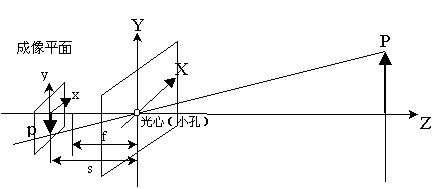
\includegraphics[width=.7\linewidth]{pinhole.jpeg}
  \caption{小孔成像原理示意图}
  \label{fig:pinhole}
\end{figure}

考虑到相机将图片从CMOS中读取出来制成完整图片时,xy方向会有不同程度的拉伸,因此,我们分别
使用两个参数$f_x, f_y$ 表示x方向和y方向上的光心,正常情况下,$f_x f_y$ 即使相互不同也不应当
相差太大。另外,在从相机坐标向图片坐标转换时,需要将像平面上的点统一平移一个便宜量,
这样使得所有像点在图片中的坐标均大于0。因此,假设我们有一3维世界坐标点[X, Y, Z],在
图片中对应的图像坐标为[u, v],则二者之间的转换可表示为:

\begin{equation}
  \begin{cases}
    u = f_x * \frac{X}{Z} + c_x \\
    v = f_y * \frac{Y}{Z} + c_y
  \end{cases}
\end{equation}


经过整理可得到较为方便书写的版本:

$$
\begin{bmatrix}
u \\
v \\
1
\end{bmatrix}
= \frac{1}{Z}
\begin{bmatrix}
  f_x & 0   & c_x \\
    0 & f_y & c_y \\
    0 & 0   &   1
\end{bmatrix}
\begin{bmatrix}
X \\
Y \\
Z
\end{bmatrix}
$$

\textbf{一种通用的相机校准模型——Kannala Brant模型}

如\ref{subsec:pinhole_cam}所示,理想状态下,图片中记录下来的物体形状
应当与真实世界中的物体满足相似关系,但是由于相机透镜的工艺、相机装配
时的误差,真实相机获取的图片中会发生畸变。Kannala Brant模型
\cite{kannala2006generic} 提供了一种较为普遍且有效的畸变拟合手段,在
工程实践中被广泛的应用在窄视角以及鱼眼相机的正畸过程中。

按照畸变产生的效果来分,主要存在两种畸变,分别是径向畸变及切向畸变。

径向畸变产生的主要原因为相机透镜的折射率无法做到完全一致,径向畸变是
以图像中心为中心,按点到中心的绝对距离r为半径对称分布的,一般来说,径向
畸变有桶型和枕型两种,两种畸变如图\ref{fig:radial_distort}所示。尽管
两种径向畸变在表现上 不太一样,但是在使用Kannala Brant模型时,可以
使用同一种近似手段来拟合两种畸变。

\begin{figure}[h] % use float package if you want it here
  \centering
  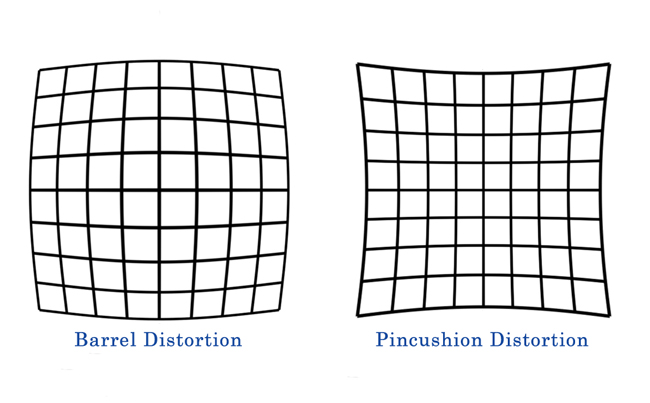
\includegraphics[width=240pt]{camera_distortion.jpg}
  \caption{左桶型畸变 右枕型畸变}
  \label{fig:radial_distort}
\end{figure}

切向畸变则是由于相机装配过程中,相机透镜平面与CMOS感光平面不完全平行造成
的,具体造成原因如图\ref{fig:tangential_distort}所示。尽管在各种相机校准
方法中,关于切向畸变 都有对应的处理手段,但是在实际工程应用中,由于切向
畸变一般较小,影响也 较小,因此大多数情况下都不予处理。Tinker的标准
校准流程中,对切向 畸变也不予处理。

\begin{figure}[h] % use float package if you want it here
  \centering
  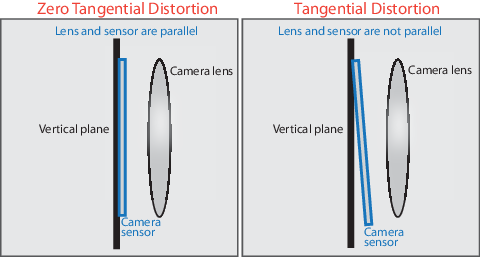
\includegraphics[width=300pt]{tangential_dist.png}
  \caption{左正常装配结果 右有装配误差的装配结果}
  \label{fig:tangential_distort}
\end{figure}

Kannala Brant模型使用光线的入射角$\theta$对图片上对应点的径向距离r进行拟合,
拟合形式如下式所示。

\begin{equation}
  r(\theta) = k_1\theta + k_2\theta^{3} + k_3\theta^{5} + k_4\theta^{7} + ...
\end{equation}

根据工程实践经验,使用KB模型校准时,将$k_1$取为1,并对
拟合参数{k}取到5阶,即有效畸变参数为$[k_2, k_3, k_4, k_5]$。如图TODO为Tinker
顶视摄像头校准前后的图片。

TODO:插入一张校准前后的图片


\subsection{导航方案的迭代}

Tinker的开发过程中一直使用ROS作为主要开发框架,而ROS的Navigation Stack中对于
导航避障提供了一套较为成熟的解决方案。Tinker前后使用了2套定位与规划算法,下面两个
章节中将对这两套方案进行详细描述。

\subsubsection{路径规划与机器人控制}

ROS的Navigation stack中提供了一整套导航避障的解决方案。其核心是同时维护地图信息
与路径规划器。地图信息使用一种分层管理的方式\cite{lu2014layered},并且分别维护
全局地图 Global Map与局部地图 Local Map。规划器也有两个,分别是Global Planner
和Local Planner。其中 Global Planner负责根据全局地图生成路径,而 Local Planner
则负责根据局部地图生成速度指令,传输给底盘执行。Tinker使用的 Global Planner是
一种基于 Dijkstra算法\cite{deng2012fuzzy}的路径生成方法,Local Planner是
一种基于dynamic window approach的速度生成方案\cite{fox1997dynamic}。上述
方案均为机器人导航领域较为经典且通用的方案,Tinker团队对上述算法进行了一些微调,以
使算法在Tinker平台上有更好的表现,如图\ref{nav_costmap}所示为Tinker进行导航任
务时可视化的调试信息。

\begin{figure}[h] % use float package if you want it here
  \centering
  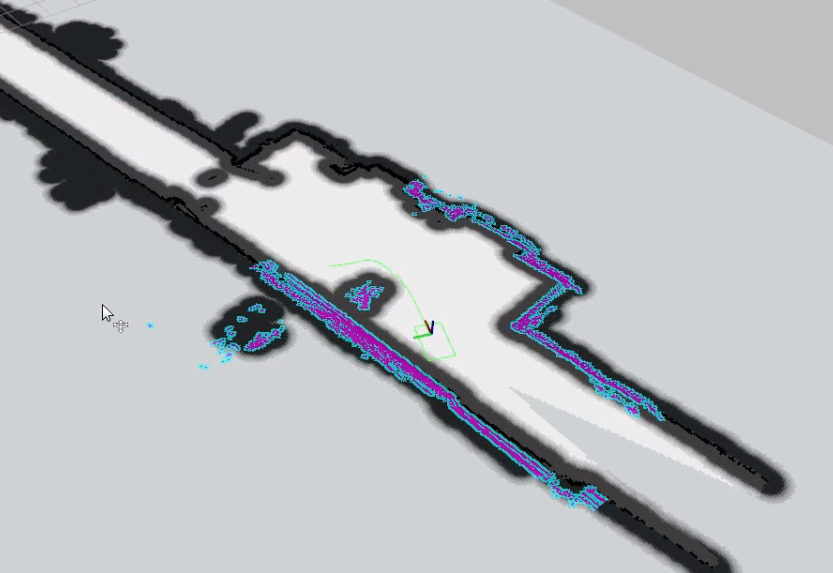
\includegraphics[width=300pt]{nav_costmap.png}
  \caption{进行导航任务时的地图与路径}
  \label{fig:nav_costmap}
\end{figure}


值得一提的是Tinker团队不断探索发现,在底盘接受速度命令端加一个smoother对临近的
几帧速度命令进行一定程度的加权平滑能够使机器人的运动性能得到质的提升。这一发现也提示
我们对于机器人这一复杂系统来说,提升整体性能的手段是多元的,在制定方案时应勇于尝试
多做实验,积极尝试各种想法,这样有助于我们使用较低的成本达到更好的性能。

\subsubsection{SLAM方案的迭代与性能分析}

Tinker最初使用的是建图与定位分开实现的方案。建图方面,我们使用 gmapping算法\cite{grisettiyz2005improving},
依赖2个北洋UTM-30LX单线激光雷达拼接定位(如图\ref{fig:utm30lx})。定位
方面,我们使用基于蒙特卡罗的
amcl算法\cite{fox2002kld}。amcl需要在地图已经给出的情况下进行定位,在
真实赛场上,比赛场景多数情况下是确定的,因此这套方案还基本可用,Tinker团队
会在开赛前对赛场进行扫描,将地图场景保存起来,之后比赛过程中单纯使用amcl
进行定位。后期随着团队成员对这套定位算法越来越熟悉,我们会将场景内可能出现
在单线雷达视野内的一切固定障碍的尺寸量下来,使用绘图软件对地图进行重建,然后
使用amcl进行定位,可以拿到更好的定位效果。

\begin{figure}
  \centering
  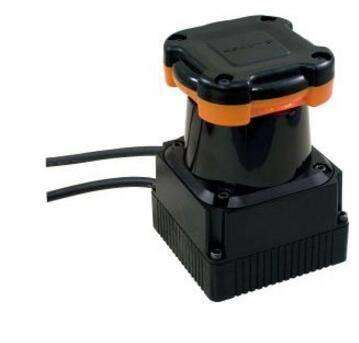
\includegraphics[width=300pt]{utm30lx.jpeg}
  \caption{北洋UTM-30LX单线激光雷达}
  \label{fig:utm30lx}
\end{figure}


虽然上述方案在长时间内被证明是稳定可用的,但是随着SLAM社区的不断发展,基于
粒子滤波的定位建图算法已经过时了,尤其是Google开源其自主开发的Cartographer
雷达建图定位算法\cite{hess2016real}之后,Tinker团队后期也将定位方案迁移为Cartographer+
ROS Navigation的模式,在更换建图定位算法之后,配合我们对Tinker硬件的二次
改版,我们也将原有的2个单线雷达减少为一个,变动之后定位数据减少,运算效率也
得到了提升。Cartographer的算法框架如图\ref{fig:cartographer}所示。

\begin{figure}[h] % use float package if you want it here
  \centering
  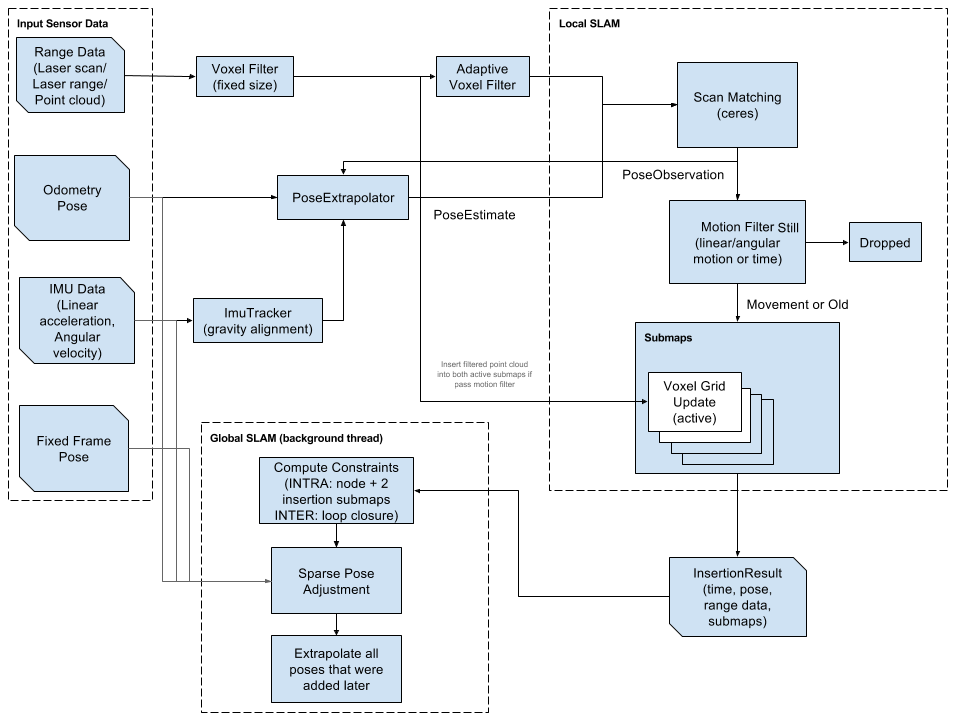
\includegraphics[width=300pt]{cartographer.png}
  \caption{Cartographer的算法框架}
  \label{fig:cartographer}
\end{figure}

\subsection{抓取方案与环境维护}

Tinker早期使用自制机械臂时结构极为简单,因此使用的机械臂控制算法也是自行
开发的,当然也完全没有环境维护及避障的意识和需要。16年之前,赛场上的抓取任务都是十分
简单的,使用恰当的运动规划并且硬编码一部分环境参数即可完成任务。在Tinker改版
使用成品机械臂之后,机械臂自由度提高,规划变得困难,此时Tinker团队经过调研
选择了基于ROS的开源机械臂规划框架MoveIt!\ref{chitta2012moveit}。新机械臂
和新框架的引入对机器人的开发造成了一定程度的冲击,在2019年的赛场上Tinker的
表现并不理想。但经过几个月的整合,Tinker团队作为清华大学孙富春教授团队的一部分
参加IROS 2019“抓取与操作”比赛,在其中取得了不错的成绩。图\ref{fig:iros}
为Tinker在IROS比赛中完成复杂的“舀抹茶”任务的场景。

\begin{figure}
  \centering
  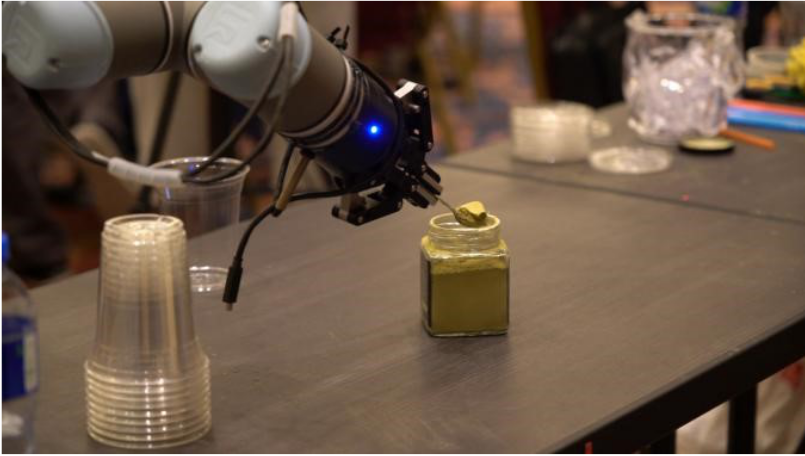
\includegraphics[width=300pt]{iros.png}
  \caption{Tinker在IROS赛场上}
  \label{fig:iros}
\end{figure}


\subsection{基于视觉的感知方案}

\subsection{语音交互方案的迭代}

Tinker团队在语音交互方面一直存在短板,语音方案的选择也是几经变换。语音交互任务
对RoboCup而言,可以粗略的划分为语音识别与语音合成两个部分。至于语音识别之后的
分析与处理过程,在RoboCup的赛场上要求极低,使用简单的正则匹配即可满足需求。

语音识别方案早期Tinker尝试过几大开源语音识别方案包括CMUsphinx\ref{lamere2003cmu},
kaldi\ref{povey2011kaldi},DeepS




























